\chapter{PENGENALAN ANTARMUKA DAN MENAMBAHKAN DATA SIG PADA APLIKASI QGIS}

Pada Bab ini kita akan mengenal bagian-bagian dasar yang biasa digunakan untuk membuat peta menggunakan QGIS 2.14, menambahkan data, dan mengeksplor data menggunakan \textit{tools-tools} yang tersedia.

\begin{enumerate}[A.]

\item \textbf{Pengenalan Antarmuka QGIS 2.14 Essen}

Bagian-bagian dari antarmuka QGIS ini seperti terlihat pada gambar \ref{fig:bagianui}.

\begin{figure}[H]
  \centering
  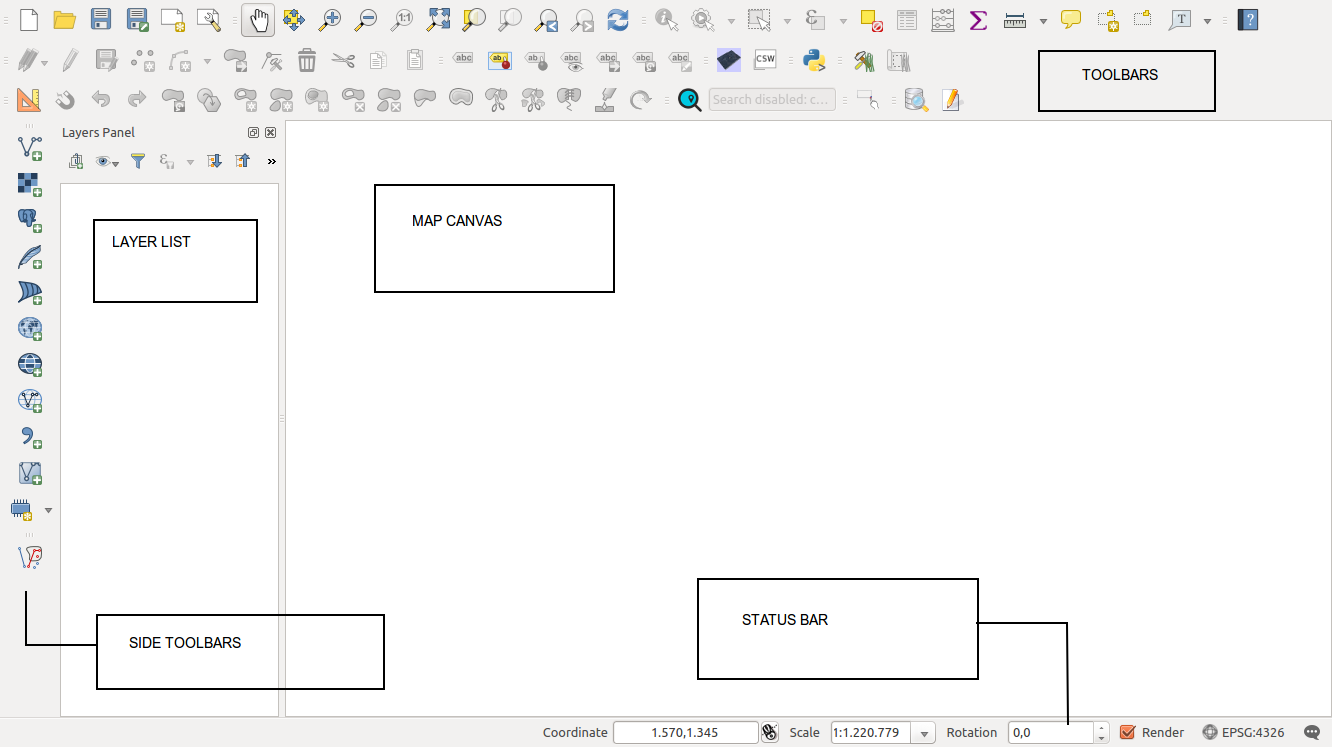
\includegraphics[width=1\textwidth]{./resources/004-bagian-qgis}
  \caption{Bagian Antarmuka QGIS}
  \label{fig:bagianui}
\end{figure}

\begin{itemize}

\item \textbf{Map Canvas}

Merupakan tempat menampilkan proyek / peta yang sedang dijalankan.

\item \textbf{Layer List}

Memuat daftar \textit{layer-layer} yang digunakan dalam proyek. Urutan \textit{layer} yang ditampilkan pada \textit{map canvas} berdasarkan urutan dari atas ke bawah pada \textit{layer list}-nya.

\item \textbf{Menu}

Bagian \textit{menu} ini tidak terlihat di gambar karena konfigurasi tampilan \textit{menu} menempel pada \textit{menu bar desktop}. \textit{Menu} ini berisi sekumpulan perintah teks untuk melakukan tugas-tugas tertentu.

\item \textbf{Toolbar dan Side Tooldbar}

Bagian ini berisi sekumpulan perintah berbasis tombol / ikon untuk melakukan tugas-tugas tertentu. \textit{Tools} dikelompokan dalam grup-grup \textit{toolbar} seperti \textit{File Toolbar}, \textit{Digitizing Toolbar}, \textit{Managed Layers Toolbar}, dan lainnya.

\item \textbf{Status Bar}

\textit{Status bar} memuat koordinat berdasarkan lokasi kursor / pointer, skala, dan sistem koordinat proyek pada \textit{map canvas}.

\end{itemize}

\item \textbf{Menambahkan Data}

Dalam QGIS dan aplikasi GIS pada umumnya, data vektor dalam format \textit{shapefile} dan data \textit{raster} yang akan ditambahkan untuk membuat sebuah \textit{project} (\texttt{*.qgis}) yang telah dibuat, melainkan hanya menyimpan \textit{style} dari data tersebut. Data tetap berada pada \textit{direktori} tempat menyimpan data, oleh karena itu satu \textit{dataset} dapat digunakan untuk berbagai \textit{project}. Berikut langkah-langkah yang dilakukan untuk menambahkan data sebagai \textit{layer} dalam QGIS.

\begin{enumerate}[1.]
  \item Klik \textit{tool} \texttt{Add Vector Layer} yang terlihat seperti pada gambar \ref{fig:addvectorlayer}.
  
\begin{figure}[H]
  \centering
  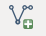
\includegraphics[scale=1]{./resources/005-ikon-add-vektor-layer}
  \caption{Ikon \textit{Add Vector Layer}}
  \label{fig:addvectorlayer}
\end{figure}

  \item Sebuah kotak dialog tempat untuk memilih \textit{file} yang akan ditambahkan ke dalam proyek QGIS akan muncul seperti pada gambar \ref{fig:addvectorlayerwindow}
  
\begin{figure}[H]
  \centering
  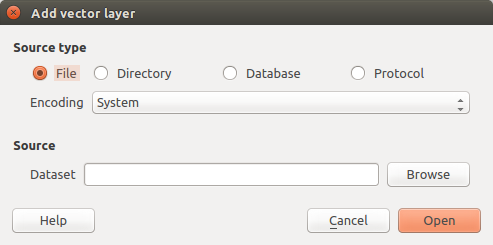
\includegraphics[scale=0.8]{./resources/006-add-vector-layer-window}
  \caption{Jendela \textit{Add Vector Layer}}
  \label{fig:addvectorlayerwindow}
\end{figure}

  \item Klik \textit{Browse} dan navigasikan pada \textit{direktori} tempat anda menyimpan \textit{shapefile}, tampilannya akan terlihat seperti gambar \ref{fig:pemilihanfilepeta}.
  
\begin{figure}[H]
  \centering
  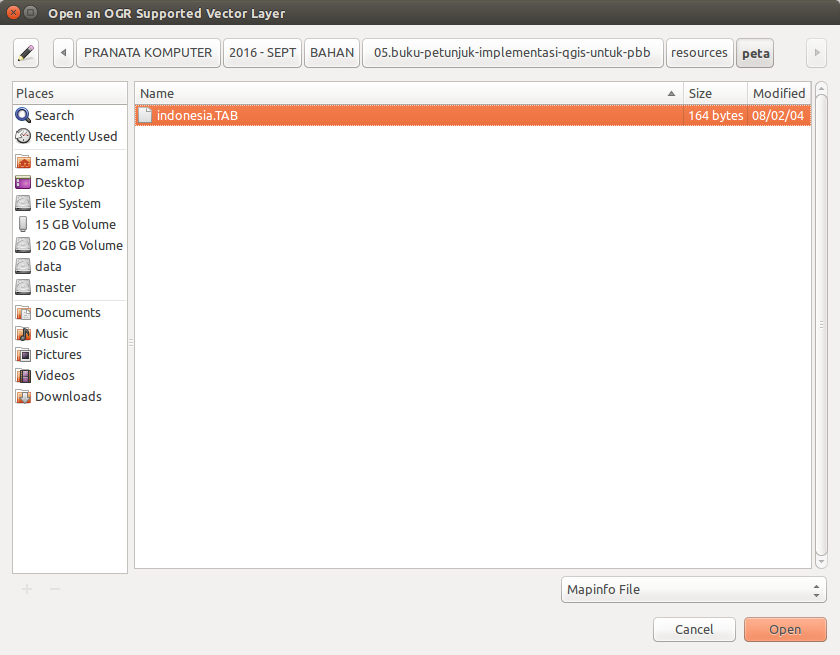
\includegraphics[width=1\textwidth]{./resources/007-pemilihan-file-peta}
  \caption{Pemilihan Layer Peta}
  \label{fig:pemilihanfilepeta}
\end{figure}

  \item Setelah memilih \textit{shapefile} yang diinginkan untuk dilihat atau diubah, klik \textit{Open} untuk memasukkan \textit{path file} ke dalam \textit{form} isian, dan klik \textit{Open} lagi pada dialog \textit{Add Vector Layer} untuk memuatnya ke dalam aplikasi. Seharusnya akan terlihat pada \textit{map canvas} seperti tampilan pada gambar \ref{fig:petaindonesiaload}
  
\begin{figure}[H]
  \centering
  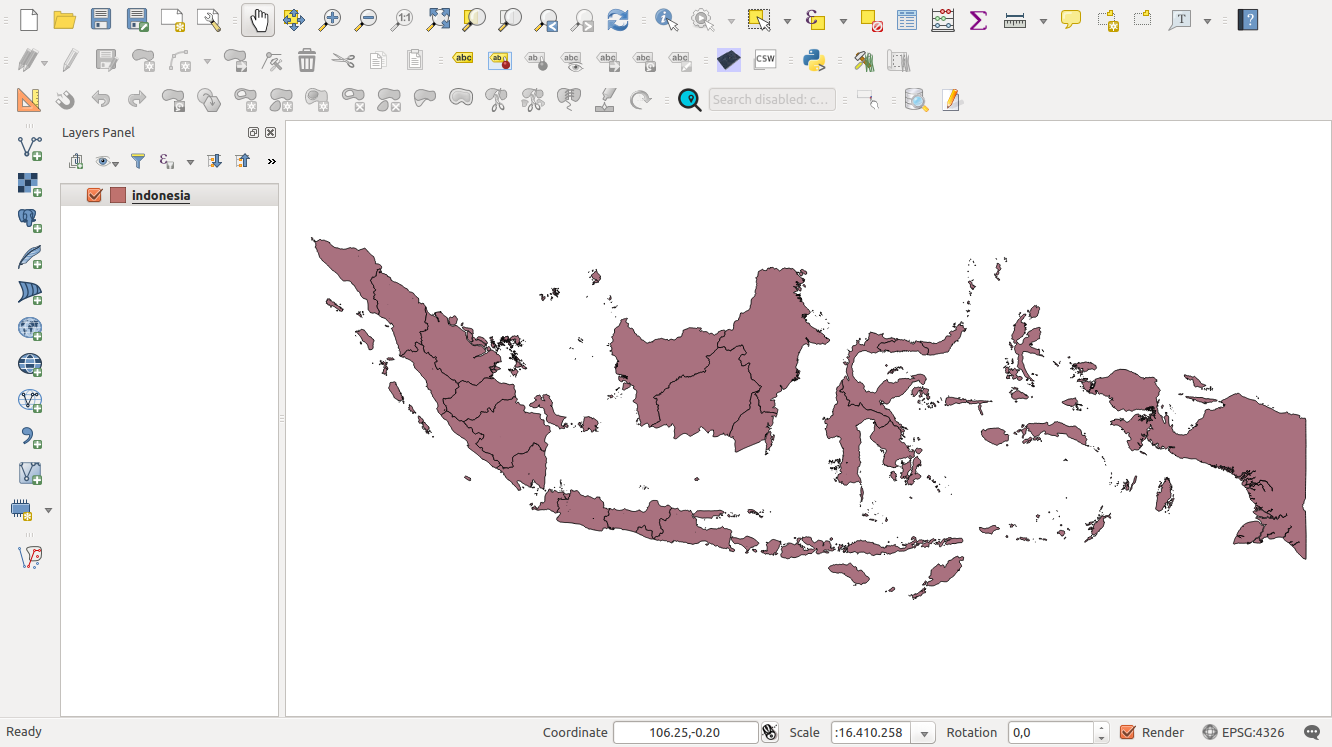
\includegraphics[width=1\textwidth]{./resources/008-peta-indonesia}
  \caption{Peta Indonesia Yang Sudah Termuat Dalam \textit{Map Canvas}}
  \label{fig:petaindonesiaload}
\end{figure}

\end{enumerate}

\item \textbf{Mengeksplor Data}

Selain menampilkan peta, \textit{layer} yang ditambahkan dapat di \textit{explore} dengan cara :

\begin{enumerate}[1.]
  \item Menavigasikan Peta
  
Kontrol utama untuk menggerakan peta dan memperbesar serta memperkecil peta berada pada \textit{Map Navigator Toolbar} seperti yang terlihat seperti gamber \ref{fig:mapnavigatortoolbar}

\begin{figure}[H]
  \centering
  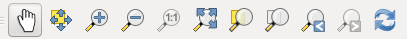
\includegraphics[scale=1]{./resources/009-map-navigator-toolbar}
  \caption{Tampilan \textit{Map Navigator Toolbar}}
  \label{fig:mapnavigatortoolbar}
\end{figure}

  \begin{itemize}
  
    \item Pilih \textit{tool} pertama yang terlihat seperti tangan. Sekarang tahan tombol \textit{mouse} sebelah kiri dan geser \textit{mouse} di dalam jendela peta. \textit{Tool} ini berfungsi untuk menggeser peta, atau menggerakannya.
    
    \item \textit{Tool} yang kedua berfungsi untuk menggeser peta menuju fitur yang terseleksi.
    
    \item \textit{Tool} ketiga yang terlihat tanda plus di dalam kaca pembesar, berguna untuk melakukan perbesaran pada peta. Pilih tombol ini, kemudian dengan menggunakan \textit{mouse}, gambar sebuah kotak sekitar area yang hendak diperbesar, dan lepas tombol \textit{mouse}.
    
    \item \textit{Tool} keempat, yang terlihat ada tanda minus di dalam kaca pembesar, berguna untuk memperkecil tampilan peta. Pilih \textit{tool} ini dan klik pada peta.
    
    \item \textit{Tool} yang terlihat tanda kaca pembesar dengan angka \texttt{1:1} berfungsi untuk perbesaran sesuai ukuran sebenarnya, yaitu dengan skala 1:1.
    
    \item \textit{Tool} yang terlihat tanda anak panah ke segala arah pada kaca pembesar berguna untuk melakukan perbesaran penuh pada peta. Ketika mengklik tombol ini, kita dapat melihat keseluruhan data yang telah kita muat di \textit{project}.
    
    \item \textit{Tool} yang terlihat tanda kaca pembesar dengan kotak berwarna kuning berfungsi untuk melakukan perbesaran pada bidang objek yang terpilih dengan menggunakan ikon seperti pada gambar \ref{fig:selectfeatureicon}
    
\begin{figure}[H]
  \centering
  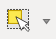
\includegraphics[scale=1]{./resources/010-select-feature-icon}
  \caption{Ikon Pemilihan Fitur}
  \label{fig:selectfeatureicon}
\end{figure}

    \item \textit{Tool} selanjutnya yang terlihat tanda kaca pembesar dengan kotak berwarna abu-abu berfungsi untuk melakukan perbesaran pada \textit{layer}/lapisan terpilih. Perbedaannya dengan \textit{tool} bergambar kaca pembesar dan tanda panah ke segala arah (kita sebut saja dengan \textit{Zoom Full}) adalah bahwa \textit{Zoom Full} akan melakukan perbesaran untuk seluruh \textit{layer} yang termuat pada \textit{Map Canvas} sedangkan \textit{tool Zoom to Selection} hanya melakukan perbesaran pada \textit{layer} yang terpilih saja.
    
    \item \textit{Tool} berikutnya adalah kaca pembesar dengan tanda panah ke kiri yang dinamakan \textit{Zoom Last}, berfungsi sebagai alat untuk melakukan perbesaran ke situasi sebelumnya. 
    
    \item \textit{Tool} berikutnya adalah kaca pembesar dengan tanda panah ke kanan yaang dinamakan \textit{Zoom Next}, berfungsi sebagai alat untuk melakukan perbesaran ke situasi setelahnya, tentunya \textit{tool} ini tidak akan aktif bila kita masih dalam kondisi perbesaran terakhir.
 
  \end{itemize}
  
  \item Identifikasi Fitur
  
  \begin{itemize}
  
    \item Untuk melihat atribut dari sebuah fitur, kita perlu memilih \textit{layer} yang kita inginkan di sebelah kiri, kemudian klik sebuah objek menggunakan \textit{tool Identify Features} dengan simbol \textit{tool} seperti gambar \ref{fig:identifyfeaturesicon}:
    
    \begin{figure}[H]
      \centering
      
\includegraphics[scale=1]{./resources/011-identify-features-icon}
      \caption{Ikon Identifikasi Fitur}
      \label{fig:identifyfeaturesicon}
    \end{figure}
    
    \item Klik pada \textit{layer} indonesia pada \textit{panel} di sebelah kiri. Kemudian pada \textit{panel} atas QGIS, klik pada \textit{tool Idnetify Features} seperti pada gambar \ref{fig:identifyfeaturesicon}.
    
    \item Sekarang pada \textit{layer} indonesia, klik pada fitur dimana saja pada peta. Ketika mengklik sebuah fitur poligon, sebuah jendela akan muncul dan menampilkan atribut dari fitur tersebut seperti diperlihatkan pada gambar \ref{fig:sampleidentifyfeature}
    
    \begin{figure}[H]
      \centering
      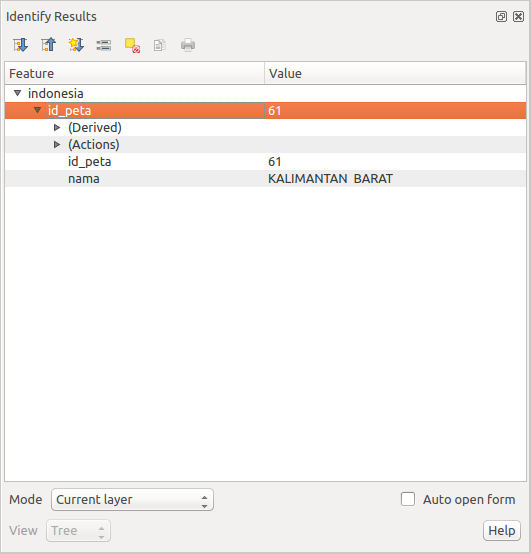
\includegraphics[scale=1]{./resources/012-sample-identify-feature}
      \caption{Contoh Jendela Atribut dari sebuah fitur}
      \label{fig:sampleidentifyfeature}
    \end{figure}
  
  \end{itemize}
  
  \item Memeriksa Atribut
  
  Memeriksa fitur individu adalah sangat berguna, tetapi bagaimana jika kita ingin melihat atribut untuk semua fitur dalam sebuah \textit{layer}? Cara yang dapat dilakukan yaitu :
  
  \begin{itemize}
  
    \item Pada \textit{panel layer} di sebelah kiri QGIS, klik kanan pada \textit{layer} lalu klik \textit{Open Attribute Table} seperti ditunjukkan pada gambar \ref{fig:menuopenattributetable}
    
    \begin{figure}[H]
      \centering
      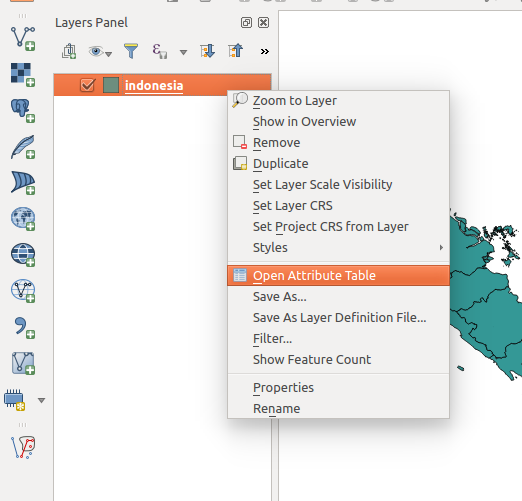
\includegraphics[scale=1]{./resources/013-menu-atribut-tabel}
      \caption{Menu Untuk Membuat Tabel Atribut}
      \label{fig:menuopenattributetable}
    \end{figure}
    
    \item Seharusnya akan tampil sebuah jendela yang terlihat seperti \textit{spreadsheet} (tabel \textit{excel}), seperti ditunjukkan pada gambar \ref{fig:attributetable}. Ini merupakan sebuah daftar dari semua fitur yang terkandung pada \textit{layer}, berikut dengan semua atribut mereka.
    
    \begin{figure}[H]
      \centering
      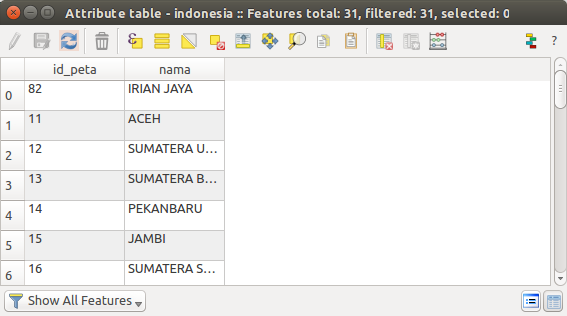
\includegraphics[scale=1]{./resources/014-tabel-atribut}
      \caption{Tabel Atribut}
      \label{fig:attributetable}
    \end{figure}
  
  \end{itemize}
  
\end{enumerate}

\end{enumerate}